\documentclass[11pt,oneside]{article}

\pdfminorversion=7
\usepackage{QuizStyle}

\hypersetup{
    pdftitle={20260929 Quiz for MATH230 Probability \& Statistics},
    pdfauthor={Jungwoo Kim},
    pdfsubject={Quiz for MATH230 Probability \& Statistics},
    pdfcreator={LaTeX}
}

\begin{document}

\quiztitle{20260929 Quiz}

\begin{exercise}{4.1}
The probability distribution of $X$, the number of imperfections per 10 meters of a synthetic fabric in continuous rolls of uniform width, is given in Exercise 3.13 on page 112 as
\[
\begin{array}{c@{\qquad}ccccc}
\toprule
x & 0 & 1 & 2 & 3 & 4 \\
\midrule
f(x) & 0.41 & 0.37 & 0.16 & 0.05 & 0.01 \\
\bottomrule
\end{array}
\]
Find the average number of imperfections per 10 meters of this fabric.
\end{exercise}

\begin{solution}
By the definition of expectation,
\[
\begin{aligned}
    \Exp[X]
    &=\sum_x x f(x) \\
    &=(0)(0.41)+(1)(0.37)+(2)(0.16)+(3)(0.05)+(4)(0.01) \\
    &=\boxed{0.88}.
\end{aligned}
\]
Thus, the average number of imperfections is $0.88$ per 10 meters of fabric.
\end{solution}

\begin{exercise}{4.2}
The probability distribution of the discrete random variable, $X$, is
\[
    f(x)=\binom{5}{x}\left(\frac14\right)^x
    \left(\frac34\right)^{5-x},
    \qquad x=0,1,2,3,4,5.
\]
Find the mean of $X$.
\end{exercise}

\begin{solution}
Using the given probability distribution,
\[
\begin{aligned}
    \Exp[X]
    &=\sum_{x=0}^{5}x f(x) \\
    &=\frac{1(405)+2(270)+3(90)+4(15)+5(1)}{1024} \\
    &=\boxed{\frac54}.
\end{aligned}
\]
Hence, $\mu_X=5/4$.
\end{solution}

\begin{exercise}{4.5}
In a gambling game, a woman is paid $\$2$ if she draws a jack or a queen and $\$4$ if she draws a king or an ace from an ordinary deck of 52 playing cards. If she draws any other card, she loses. How much should she pay to play if the game is fair?
\end{exercise}

\begin{solution}
There are $8$ jacks or queens and $8$ kings or aces. Thus the expected payout is
\[
    \Exp[X]
    =2\left(\frac{8}{52}\right)
    +4\left(\frac{8}{52}\right)
    =\frac{12}{13}\approx0.92.
\]
For a fair game, the entry fee must equal the expected payout. Therefore, she should pay
\[
    \boxed{\$0.92}\quad\text{(approximately)}.
\]
\end{solution}

\begin{exercise}{4.7}
By investing in a particular stock, a person can make a profit in one year of $\$4000$ with probability $0.3$ or take a loss of $\$1000$ with probability $0.7$. What is this person's expected gain?
\end{exercise}

\begin{solution}
Let $X$ denote the gain, so a loss is represented by a negative value. Then
\[
    \Exp[X]=(4000)(0.3)+(-1000)(0.7)=\boxed{\$500}.
\]
\end{solution}

\begin{exercise}{4.9}
A private pilot wishes to insure an airplane for $\$200{,}000$. The insurance company estimates that a total loss will occur with probability $0.001$, a 50\% loss with probability $0.01$, and a 25\% loss with probability $0.2$. Ignoring all other partial losses, what premium should the insurance company charge each year to realize an average profit of $\$500$?
\end{exercise}

\begin{solution}
Let $L$ be the insurer's loss payment. Its expected value is
\[
\begin{aligned}
    \Exp[L]
    &=(200000)(0.001)+(100000)(0.01)+(50000)(0.2) \\
    &=11200.
\end{aligned}
\]
If $p$ is the annual premium, an average profit of $\$500$ requires
\[
    p-11200=500.
\]
Hence,
\[
    \boxed{p=\$11{,}700}.
\]
\end{solution}

\begin{exercise}{4.10}
Two tire-quality experts examine stacks of tires and assign a quality rating to each tire on a 3-point scale. Let $X$ denote the rating given by expert A and $Y$ denote the rating given by B. The following table gives the joint distribution for $X$ and $Y$.
\[
\begin{array}{c@{\qquad}ccc}
\toprule
f(x,y) & \multicolumn{3}{c}{y} \\
\cmidrule(lr){2-4}
x & 1 & 2 & 3 \\
\midrule
1 & 0.10 & 0.05 & 0.02 \\
2 & 0.10 & 0.35 & 0.05 \\
3 & 0.03 & 0.10 & 0.20 \\
\bottomrule
\end{array}
\]
Find $\mu_X$ and $\mu_Y$.
\end{exercise}

\begin{solution}
From the joint distribution, the marginal probabilities are
\[
\begin{aligned}
    p_X(1)&=0.17, & p_X(2)&=0.50, & p_X(3)&=0.33,\\
    p_Y(1)&=0.23, & p_Y(2)&=0.50, & p_Y(3)&=0.27.
\end{aligned}
\]
Therefore,
\[
\begin{aligned}
    \mu_X=\Exp[X]&=(1)(0.17)+(2)(0.50)+(3)(0.33)=2.16,\\
    \mu_Y=\Exp[Y]&=(1)(0.23)+(2)(0.50)+(3)(0.27)=2.04.
\end{aligned}
\]
Hence,
\[
    \boxed{\mu_X=2.16,\qquad \mu_Y=2.04}.
\]
\end{solution}

\begin{exercise}{4.13}
The density function of the continuous random variable $X$, the total number of hours, in units of 100 hours, that a family runs a vacuum cleaner over a period of one year, is given in Exercise 3.7 on page 112 as
\[
    f(x)=
    \begin{cases}
        x, & 0<x<1,\\
        2-x, & 1\leq x<2,\\
        0, & \text{elsewhere}.
    \end{cases}
\]
Find the average number of hours per year that families run their vacuum cleaners.
\end{exercise}

\begin{solution}
Since $X$ is measured in units of 100 hours,
\[
\begin{aligned}
    \Exp[X]
    &=\int_0^1 x\,f(x)\,\dd x+\int_1^2 x\,f(x)\,\dd x \\
    &=\int_0^1 x^2\,\dd x+\int_1^2 x(2-x)\,\dd x \\
    &=1.
\end{aligned}
\]
Thus the average running time is
\[
    \boxed{100\text{ hours per year}}.
\]
\end{solution}

\begin{exercise}{4.17}
Let $X$ be a random variable with the following probability distribution:
\[
\begin{array}{c@{\qquad}ccc}
\toprule
x & -3 & 6 & 9 \\
\midrule
f(x) & \frac16 & \frac12 & \frac13 \\
\bottomrule
\end{array}
\]
Find $\mu_{g(X)}$, where $g(X)=(2X+1)^2$.
\end{exercise}

\begin{solution}
By the expectation formula for a function of a discrete random variable,
\[
\begin{aligned}
    \mu_{g(X)}=\Exp[g(X)]
    &=25\left(\frac16\right)
      +169\left(\frac12\right)
      +361\left(\frac13\right) \\
    &=\boxed{209}.
\end{aligned}
\]
\end{solution}

\begin{exercise}{4.18}
Find the expected value of the random variable $g(X)=X^2$, where $X$ has the probability distribution of Exercise 4.2.
\end{exercise}

\begin{solution}
Using the distribution from Exercise 4.2 directly,
\[
\begin{aligned}
    \Exp[X^2]
    &=\sum_{x=0}^{5}x^2 f(x) \\
    &=\frac{1^2(405)+2^2(270)+3^2(90)+4^2(15)+5^2(1)}{1024} \\
    &=\boxed{\frac52}.
\end{aligned}
\]
\end{solution}

\begin{exercise}{4.19}
A large industrial firm purchases several new computers at the end of each year, the exact number depending on the frequency of repairs in the previous year. Suppose that the number of computers, $X$, purchased each year has the following probability distribution:
\[
\begin{array}{c@{\qquad}cccc}
\toprule
x & 0 & 1 & 2 & 3 \\
\midrule
f(x) & \frac{1}{10} & \frac{3}{10} & \frac25 & \frac15 \\
\bottomrule
\end{array}
\]
If the cost of the desired model is $\$1200$ per unit and at the end of the year a refund of $50X^2$ dollars will be issued, how much can this firm expect to spend on new computers during this year?
\end{exercise}

\begin{solution}
If $g(X)$ is the net expenditure, then
\[
    g(X)=1200X-50X^2.
\]
Thus,
\[
\begin{aligned}
    \Exp[g(X)]
    &=(0)\left(\frac{1}{10}\right)
      +(1150)\left(\frac{3}{10}\right)
      +(2200)\left(\frac25\right)
      +(3150)\left(\frac15\right) \\
    &=\boxed{\$1855}.
\end{aligned}
\]
\end{solution}

\begin{exercise}{4.20}
A continuous random variable $X$ has the density function
\[
    f(x)=
    \begin{cases}
        \dfrac12 e^{-x/2}, & x>0,\\
        0, & \text{elsewhere}.
    \end{cases}
\]
Find the expected value of $g(X)=e^{X/4}$.
\end{exercise}

\begin{solution}
By the expectation formula for a function of a continuous random variable,
\[
\begin{aligned}
    \Exp[g(X)]
    &=\int_0^\infty e^{x/4}\left(\frac12e^{-x/2}\right)\dd x \\
    &=\frac12\int_0^\infty e^{-x/4}\,\dd x \\
    &=\boxed{2}.
\end{aligned}
\]
\end{solution}

\begin{exercise}{4.23}
Suppose that $X$ and $Y$ have the following joint probability function $f(x,y)$:
\[
\begin{array}{c@{\qquad}cc}
\toprule
f(x,y) & \multicolumn{2}{c}{x} \\
\cmidrule(lr){2-3}
y & 2 & 4 \\
\midrule
1 & 0.15 & 0.10 \\
3 & 0.25 & 0.25 \\
5 & 0.15 & 0.10 \\
\bottomrule
\end{array}
\]
\begin{exercisesubparts}
    \item Find the expected value of $g(X,Y)=XY^2$.
    \item Find $\mu_X$ and $\mu_Y$.
\end{exercisesubparts}
\end{exercise}

\begin{solution}
\noindent\textup{(a)} By the expectation formula for a function of two discrete random variables,
\[
\begin{aligned}
    \Exp[XY^2]
    &=\sum_x\sum_y xy^2f(x,y) \\
    &=(2)(1)^2(0.15)+(4)(1)^2(0.10)
      +(2)(3)^2(0.25)+(4)(3)^2(0.25)\\
    &\qquad +(2)(5)^2(0.15)+(4)(5)^2(0.10) \\
    &=\boxed{31.7}.
\end{aligned}
\]

\medskip
\noindent\textup{(b)} The marginal probabilities are
\[
    p_X(2)=0.55,\qquad p_X(4)=0.45,
\]
and
\[
    p_Y(1)=0.25,\qquad p_Y(3)=0.50,\qquad p_Y(5)=0.25.
\]
Hence,
\[
\begin{aligned}
    \mu_X&=\Exp[X]=(2)(0.55)+(4)(0.45)=2.9,\\
    \mu_Y&=\Exp[Y]=(1)(0.25)+(3)(0.50)+(5)(0.25)=3.00.
\end{aligned}
\]
Therefore,
\[
    \boxed{\mu_X=2.9,\qquad \mu_Y=3.00}.
\]
\end{solution}

\begin{exercise}{4.26}
Let $X$ and $Y$ be random variables with joint density function
\[
    f(x,y)=
    \begin{cases}
        4xy, & 0<x,y<1,\\
        0, & \text{elsewhere}.
    \end{cases}
\]
Find the expected value of $Z=\sqrt{X^2+Y^2}$.
\end{exercise}

\begin{solution}
Using the joint density,
\[
\begin{aligned}
    \Exp[Z]
    &=\int_0^1\int_0^1 4xy\sqrt{x^2+y^2}\,\dd x\,\dd y \\
    &=\frac43\int_0^1 y\left[(1+y^2)^{3/2}-y^3\right]\dd y \\
    &=\frac43\left(\frac{4\sqrt2-1}{5}-\frac15\right) \\
    &=\boxed{\frac{16\sqrt2-8}{15}}.
\end{aligned}
\]
\end{solution}

\begin{exercise}{4.28}
Consider the information in Exercise 3.28 on page 113. The problem deals with the weight in ounces of the product in a cereal box, with
\[
    f(x)=
    \begin{cases}
        \dfrac25, & 23.75\leq x\leq26.25,\\
        0, & \text{elsewhere}.
    \end{cases}
\]
\begin{exercisesubparts}
    \item Plot the density function.
    \item Compute the expected value, or mean weight, in ounces.
    \item Are you surprised at your answer in (b)? Explain why or why not.
\end{exercisesubparts}
\end{exercise}

\begin{solution}
\noindent\textup{(a)} The density is constant on $[23.75,26.25]$ and zero elsewhere.

\Needspace{18\baselineskip}
\begin{center}
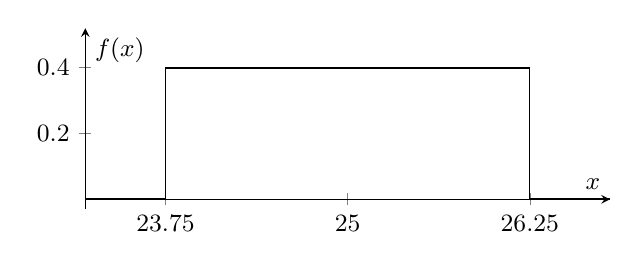
\begin{tikzpicture}
\begin{axis}[
    width=0.68\textwidth,
    height=0.32\textwidth,
    axis lines=middle,
    xmin=23.2,
    xmax=26.8,
    ymin=-0.03,
    ymax=0.52,
    xlabel={$x$},
    ylabel={$f(x)$},
    xtick={23.75,25,26.25},
    xticklabels={$23.75$,$25$,$26.25$},
    ytick={0,0.2,0.4},
    tick label style={font=\small},
    label style={font=\small},
    clip=false
]
    \addplot[black,thick] coordinates {(23.2,0) (23.75,0)};
    \addplot[black,thick] coordinates {(23.75,0.4) (26.25,0.4)};
    \addplot[black,thick] coordinates {(26.25,0) (26.8,0)};
    \addplot[black,thin] coordinates {(23.75,0) (23.75,0.4)};
    \addplot[black,thin] coordinates {(26.25,0) (26.25,0.4)};
\end{axis}
\end{tikzpicture}
\end{center}

\medskip
\noindent\textup{(b)} By the definition of expectation,
\[
\begin{aligned}
    \Exp[X]
    &=\int_{23.75}^{26.25}x\left(\frac25\right)\dd x \\
    &=\frac15\left(26.25^2-23.75^2\right) \\
    &=\boxed{25\text{ ounces}}.
\end{aligned}
\]

\medskip
\noindent\textup{(c)} No. The density is constant on an interval symmetric about $25$, so its mean is the midpoint of the interval, $25$ ounces.
\end{solution}

\end{document}
